
\documentclass[a4paper,12pt]{report}
\usepackage[utf8]{inputenc}
\usepackage{color,amsmath,xcolor,listings,graphicx}
\usepackage[francais]{babel}
%
% paramétrage pour les zones de code perl
\lstset{
    language=Perl, commentstyle=\textit, frame=shadowbox,
    rulesepcolor=\color{gray}, basicstyle=\ttfamily\small, columns=flexible,
    tabsize=3, extendedchars=true, showspaces=false,
    showstringspaces=false, numbers=left, numberstyle=\tiny,
    breaklines=true, breakautoindent=true, captionpos=b, morecomment=[l]{//}
}
%
%language=Octave %-> choose the language of the code
%basicstyle=\footnotesize %-> the size of the fonts used for the code
%numbers=left %-> where to put the line-numbers
%numberstyle=\footnotesize %-> size of the fonts used for the line-numbers
%stepnumber=2 -> the step between two line-numbers.
%numbersep=5pt -> how far the line-numbers are from the code
%backgroundcolor=\color{white} -> sets background color (needs package)
%showspaces=false -> show spaces adding particular underscores
%showstringspaces=false -> underline spaces within strings
%showtabs=false -> show tabs within strings through particular underscores
%frame=single -> adds a frame around the code
%tabsize=2 -> sets default tab-size to 2 spaces
%captionpos=b -> sets the caption-position to bottom
%breaklines=true -> sets automatic line breaking
%breakatwhitespace=false -> automatic breaks happen at whitespace
%morecomment=[l]{//} -> displays comments in italics (language dependent)
%
%
% infos du document
\title{QNAP}
\author{Boulic Guillaume, Émeric Tosi}
\date{\today}
%
%
\begin{document}
%
    \maketitle{} % Afficher la page de garde : Titre + Auteur(s) + Date de dernière compilation
%
%    \begin{figure} % on s'en fout de l'image moche, c'est juste pour test xD
%        \begin{center}
            %\includegraphics{network.png}
            %\includegraphics[height=128, width=128]{network.png}
            %\includegraphics[scale=0.5]{network.png}
%        \end{center}
%            \caption{ Laule } % ce qui apparait juste en dessous de l'image
%            \label{c'est styler !}
%    \end{figure}

    \setcounter{tocdepth}{1} % définir la profondeur de l'Index
    \renewcommand{\contentsname}{Sommaire} % renommer l'Index en Sommaire
    \tableofcontents{} % afficher l'Index
    \clearpage
%
%
% Differentes Parties / Chapitres / Autres fichiers à inclure :
%
%
%
\chapter{RTC : Réseau Téléphonique Commuté}
%
    \section{Analyse sur un lien}
        \label{seullien} % label pour reference
%
        \subsection{Énoncé}
%
            \paragraph{}
Considérons un lien d'un réseau à commutation de circuits permettant de véhiculer de la voix téléphonique.
            %    \begin{figure}
            %        \begin{center}
                        %\includegraphics[scale=0.5]{RSC/1.1.png}
            %        \end{center}
            %            \caption{ Schéma du réseau à commutation de circuit }
            %            \label{ Schéma du réseau à commutation de circuit }
            %    \end{figure}
%
            \paragraph{}
Chacune des connexions nécessite un débit de 64 Kb/s bi-directionnels.
On peut multiplexer simultanément $C$ appels téléphoniques sur ce lien.
%
        \paragraph{}
Le nombre d'utilisateurs est suffisamment grand pour supposer que les arrivées des nouveaux appels suivent une loi de paramètre, les durées des appels sont supposées suivre une loi exponentielle de paramètre , (1\u = 3 min).
%
        \subsection{Probabilité de blocage d'appel en fonction de la charge $\rho$ et de la capacité $C$}
\[ P(\text{blocage}) = \frac{ \frac{ \rho^C }{ C! } }{ \sum\limits_{i=0}^C \frac{ \rho^i }{ i! } } \]
\begin{center}
    avec $\rho$ la charge en Erlang et $C$ la capacité.
\end{center}
    % TODO >>>
    % ici graphique calcul theorique avec k et rho qui changent
    % TODO <<<
%
        \subsection{Simulation de la probabilité de blocage d'appel pour une charge comprise entre 10 et 70 Erlangs}
Blablabla 1
    % TODO >>>
    % SIMULATION
    % ici graphique
    % TODO <<<
%
        \subsection{Variation de la capacité C pour une variation de la charge normalisée entre 0.5 et 1}
    % TODO >>>
    % SIMULATION
    % ici graphique
    % TODO <<<
Blablabla 2
%
        \subsection{Comparaison des taux de blocage expérimental et théorique}
Blablabla 3
%
    \clearpage
%
%
%
    \section{Analyse sur un réseau de trois commutateurs}
%
        \subsection{Énoncé}
%
            \paragraph{}
Désormais, nous considérons le réseau composé des 3 nœuds suivant :
            %    \begin{figure}
            %        \begin{center}
                        %\includegraphics[scale=0.5]{RSC/1.2.png}
            %        \end{center}
            %            \caption{ Schéma du réseau à 3 commutateurs }
            %            \label{ Schéma du réseau à 3 commutateurs }
            %    \end{figure}
%
            \paragraph{}
Les arrivées sont supposées Poissonniennes sur chacun des nœuds et le trafic se répartit équiprobablement entre les différents nœuds.
Les durées des appels sont supposées exponentielles de même paramètre que dans la première partie (1-a).
Nous ne considérons pas les appels locaux ni les appels qui n'aboutissent pas (absence).
%
        \subsection{Probabilités de blocage avec le chemin de débordement en cas de saturation du chemin direct}
Blablabla 4
%
        \subsection{Comparaison des résultats avec la partie \ref{seullien}}
        % (on choisira donc des charges de trafic et des capacités de liens équivalentes)
Blablabla 5
    % TODO >>>
    % ici graphique simulation ou juste calculs ??
    % TODO <<<
%
        \subsection{Problèmes à très forte charge !}
            \paragraph{}
Une solution consiste à n'utiliser le chemin de débordement que lorsque celui-ci n'est pas très encombré (en dessous d'un certain seuil d'occupation sur chacun des liens).
Cela revient donc à laisser une marge M aux appels directs.
%
            \subsubsection{Commentaires}
Blablabla 6
%
            \subsubsection{Simulation en prenant une marge comprise entre 1 et 3}
Blablabla 7
    % TODO >>>
    % ici graphique simulation
    % TODO <<<
%
    \clearpage
%

\clearpage
%
%
%
\chapter{Commutation de paquets}
%
    \section{Un commutateur de paquets}
%
        \subsection{Énoncé}
%
            \paragraph{}
Nous cherchons à simuler un lien de sortie d'un commutateur de paquets.
%
            \begin{figure}[h]
                \centering
                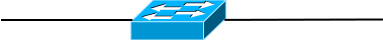
\includegraphics[scale=0.5]{RSC/2-0.png}
                \caption{ Schéma du système à commutateur de paquets étudié }
                \label{ Schema du systeme a commutateur de paquets }
            \end{figure}
%
            \paragraph{}
L'arrivée des paquets est supposée suivre une loi exponentielle de paramètre $\lambda$.
Nous positionnons une file en sortie du commutateur pour stocker les différents paquets.
Les paquets ont une longueur exponentielle-ment distribuée de paramètre $\frac{1}{\nu} = 10 000 \ \text{bits}$.
Le lien de sortie a un débit de 10 Mbit/s.
%
        \subsection{Calcul analytique du temps moyen de service $\frac{1}{\mu}$}
\[  \text{Temps moyen de service} = \frac{1}{\mu} \]
\[ \iff \frac{1}{\nu} * \frac{1}{D} = 10^{4} * \frac{1}{10^{7}} = \frac{1}{10^{3}} = 10^{-3} \ \text{seconde} \]
%
        \subsection{Déterminer le nombre moyen de paquets dans la file et le temps moyen de réponse en fonction du taux d'arrivée pour différentes durées de simulation}
%
            \begin{figure}[h]
                \centering
                
\includegraphics[scale=0.5]{RSC/2-1.png}
                \caption{ Schéma de fonctionnement d'un commutateur de paquets }
                \label{ Schema de fonctionnement d'un commutateur de paquets }
            \end{figure}
%
\[  \lambda = \rho * \mu \]
\[  \text{Charge de trafic} \ \rho = \frac{\lambda}{\mu} \]
\[  \text{Nombre moyen de client} \ \bar{N} = \frac{\rho}{(1 - \rho)} \]
\[  \text{Temps moyen de reponse} \ \bar{W} = \frac{1}{(\mu - \lambda)} \]
\[  \bar{N} = \lambda \bar{W} \]
\begin{center}
    \begin{tabular}{ | c | c| c | c | }
        \hline
            $\rho$ & 0.1 & 0.5 & 0.9 \\
        \hline
            $\lambda$ & $10^{2}$ & $5 * 10^{2}$ & $9 * 10^{2}$ \\
        \hline
            Nombre moyen de client & 0.11111 & 1 & 9 \\
        \hline
            Temps moyen de réponse [s] & 0.00111 & 0.002 & 0.01 \\
        \hline
    \end{tabular}
\end{center}
%
        \subsection{Comparaison du résultat de la simulation avec la théorie}
            \paragraph{}
Blablabla 1
\begin{figure}
    \centering
    \begin{gnuplot}[terminal=epslatex, terminaloptions=color dashed]

    set xlabel 'Charge (\%)'
    set ylabel 'Taux de rejet'
    plot "qnap/partie2/p2.q3.data" u 1:2 t "minT",\
        "qnap/partie2/p2.q3.data" u 1:3 t "maxT",\
        "qnap/partie2/p2.q3.data" u 1:4 w l t "moyenne temps traitement",\
        "qnap/partie2/p2.q3.data" u 1:5 t "minA" axes x1y2,\
        "qnap/partie2/p2.q3.data" u 1:6 t "maxA" axes x1y2,\
        "qnap/partie2/p2.q3.data" u 1:7 w l t "moyenne nb paquets en attente" axes x1y2
    \end{gnuplot}
    \caption{Résultats de la simulation.}%
    \label{pic:p2q3}%
\end{figure}
%
        \subsection{Cas où les paquets ont une longueur constante (10000 bits)}
%
            \subsubsection{Calculer analytiquement le temps moyen de service $\frac{1}{\mu}$}
%
                \paragraph{}
On obtient la même chose que précédemment :
\[  \text{Temps moyen de service} = \frac{1}{\mu} \]
\[ \iff \frac{1}{\nu} * \frac{1}{D} = 10^{4} * \frac{1}{10^{7}} = \frac{1}{10^{3}} = 10^{-3} \ \text{seconde} \]
%
            \subsubsection{Résultats en fonction du taux d'arrivée pour différentes durées de simulation}
%
% voir pour trouver des formules, la progression doit être linéaire en fonction de $\rho$.
%
                \paragraph{Temps moyen de réponse}
Blablabla 3
%
                \paragraph{Nombre moyen de paquets dans la file d'attente}
Blablabla 4
%
            \subsubsection{Analyse et comparaison des résultats}
%
                \paragraph{}
Blablabla 5
    % TODO >>>
    % SIMULATION
    % ici graphique
    % TODO <<<
\begin{figure}
    \centering
    \begin{gnuplot}[terminal=epslatex, terminaloptions=color dashed]

    set xlabel 'Charge (\%)'
    set ylabel 'Taux de rejet'
    plot "qnap/partie2/p2.cst.data" u 1:2 t "minT",\
        "qnap/partie2/p2.cst.data" u 1:3 t "maxT",\
        "qnap/partie2/p2.cst.data" u 1:4 w l t "moyenne temps traitement",\
        "qnap/partie2/p2.cst.data" u 1:5 t "minA" axes x1y2,\
        "qnap/partie2/p2.cst.data" u 1:6 t "maxA" axes x1y2,\
        "qnap/partie2/p2.cst.data" u 1:7 w l t "moyenne nb paquets en attente" axes x1y2
    \end{gnuplot}
    \caption{Résultat de la simulation pour une taille de paquet constante (10Kbits).}%
    \label{pic:p2cst}%
\end{figure}
%
    \clearpage
%

\clearpage
%
%
\chapter*{Conclusion}
\addcontentsline{toc}{chapter}{Conclusion}
        \paragraph{}
Too much bullshit here :P
    \clearpage
%
%

\appendix{}

\chapter{Annexes}

    \section{Exemple(s)}

        \paragraph{}
            \emph{emphatique}
            \textbf{gras}
            \texttt{machine à écrire}
            \textsl{incliné}
            \textsc{Petites majuscules}

        \paragraph{}
            The foundations of the rigorous study of \emph{analysis}
            were laid in the nineteenth century, notably by the
            mathematicians Cauchy and Weierstrass. Central to the
            study of this subject are the formal definitions of
            \emph{limits} and \emph{continuity}.

        \paragraph{}
            Let $D$ be a subset of $\bf R$ and let
            $f \colon D \to \mathbf{R}$ be a real-valued function on
            $D$. The function $f$ is said to be \emph{continuous} on
            $D$ if, for all $\epsilon > 0$ and for all $x \in D$,
            there exists some $\delta > 0$ (which may depend on $x$)
            such that if $y \in D$ satisfies
            \[ |y - x| < \delta \]
            then
            \[ |f(y) - f(x)| < \epsilon. \]

        \paragraph{}
            One may readily verify that if $f$ and $g$ are continuous
            functions on $D$ then the functions $f+g$, $f-g$ and
            $f.g$ are continuous. If in addition $g$ is everywhere
            non-zero then $f/g$ is continuous.

    \clearpage


%
    \section{Répétition}
%
        \paragraph{}
Implémentation de l'envoi pour le Code de Répétition
\lstinputlisting{./Repetition/Perl/receptionNoise.pl}
    \clearpage
%
        \paragraph{}
Implémentation de la réception pour le Code de Répétition
\lstinputlisting{./Repetition/Perl/envoiNoise.pl}
    \clearpage
%
        \paragraph{}
Implémentation de la vérification pour le Code de Répétition
\lstinputlisting{./Repetition/Perl/Repetition.pm}
    \clearpage


%
    \section{VRC}
%
        \paragraph{}
Implémentation de l'envoi pour le VRC
\lstinputlisting{./VRC/Perl/receptionNoise.pl}
    \clearpage
%
        \paragraph{}
Implémentation de la réception pour le VRC
\lstinputlisting{./VRC/Perl/envoiNoise.pl}
    \clearpage
%
        \paragraph{}
Implémentation de la vérification VRC
\lstinputlisting{./VRC/Perl/Parity.pm}
    \clearpage

\clearpage
%
%
%\listoffigures % index des images du rapport
%\clearpage
%
% fin
\end{document}
